\documentclass[11pt,a4paper]{article}
\usepackage[utf8]{inputenc}
\usepackage[margin=1in]{geometry}
\usepackage{graphicx}
\usepackage{tikz}
\usepackage{float}
\usepackage{tabularx}
\usepackage{hyperref}
\usepackage{xcolor}
\usepackage{listings}
\usepackage{fancyhdr}
\usepackage{multicol}

\usetikzlibrary{shapes.geometric, arrows, positioning, fit, backgrounds, shadows}

\tikzstyle{system} = [rectangle, rounded corners, minimum width=3cm, minimum height=1cm, text centered, draw=black, fill=gray!30, drop shadow]
\tikzstyle{component} = [rectangle, minimum width=2.5cm, minimum height=0.8cm, text centered, draw=black, fill=blue!10]
\tikzstyle{external} = [rectangle, minimum width=2.5cm, minimum height=0.8cm, text centered, draw=black, fill=orange!20]
\tikzstyle{process} = [rectangle, minimum width=2.5cm, minimum height=0.8cm, text centered, draw=black, fill=green!10]
\tikzstyle{decision} = [diamond, aspect=2, minimum width=2cm, minimum height=0.8cm, text centered, draw=black, fill=yellow!20]
\tikzstyle{arrow} = [thick,->,>=stealth]
\tikzstyle{line} = [thick,-]

\pagestyle{fancy}
\fancyhf{}
\rfoot{\thepage}

\title{\textbf{Case-Third-Party-Reader Technical Report}}
\author{}
\date{}

\begin{document}

\maketitle

\section*{Executive Summary}

The Case-Third-Party-Reader is a critical bidirectional synchronization service in Datadog's case management domain that enables seamless integration between Case Management and third-party ticketing systems. It consumes events from collaboration integration Kafka topics (Jira and ServiceNow webhooks) and applies validated changes to the internal Case Management system. The service implements sophisticated filtering logic to prevent synchronization loops, respects project-specific configuration, and handles custom field mappings while maintaining data consistency through optimistic locking.

\section{Service Overview}

\subsection{Primary Functions}

\begin{enumerate}    \item \textbf{Kafka Event Consumption}: Consumes events from separate Kafka topics for Jira and ServiceNow integrations
    \item \textbf{Event Decoding}: Transforms third-party webhook payloads into normalized changelog structures
    \item \textbf{Intelligent Filtering}: Two-stage filtering (PreFilter and Filter) to optimize performance and prevent sync loops
    \item \textbf{State Synchronization}: Applies validated changes to cases including title, description, priority, status, assignee, due dates, and comments
    \item \textbf{Custom Field Support}: Handles custom field mappings, particularly for Jira custom due date fields
    \item \textbf{Conflict Detection}: Validates state consistency before applying changes to prevent concurrent update conflicts
\end{enumerate}

\subsection{Supported Integrations}

\textbf{Jira}
\begin{itemize}    \item Event types: \texttt{jira:issue\_updated}, \texttt{comment\_created}
    \item Bidirectional sync for all standard fields and custom due date fields
    \item Metadata caching with 5-minute TTL for performance optimization
    \item State conflict detection for priority, status, and assignee changes
\end{itemize}

\textbf{ServiceNow}
\begin{itemize}    \item Event types: Comments (including work notes) and status changes
    \item Instance-based filtering with configuration caching
    \item Sync cycle prevention through author detection
\end{itemize}

\subsection{Key Metrics}

\begin{itemize}    \item \textbf{Deployment Flavors}: 2 separate deployments (Jira, ServiceNow)
    \item \textbf{Consumer Group}: case-management (shared with other case management consumers)
    \item \textbf{Replicas}: 1 per flavor deployment
    \item \textbf{Filter Reasons}: 27 distinct filtering reasons for comprehensive observability
    \item \textbf{Health Checks}: Liveness and readiness probes on port 8080
    \item \textbf{Deployment Environments}: Staging, Production, Government (FIPS-compliant)
\end{itemize}

\section{Architecture Overview}

\subsection{System Architecture}

The system follows a flavor-based deployment architecture where separate service instances handle different third-party integrations. Each flavor consumes from its dedicated Kafka topic and processes events according to integration-specific logic while sharing common processing patterns through abstraction interfaces.

\clearpage
\begin{figure}[H]
\centering
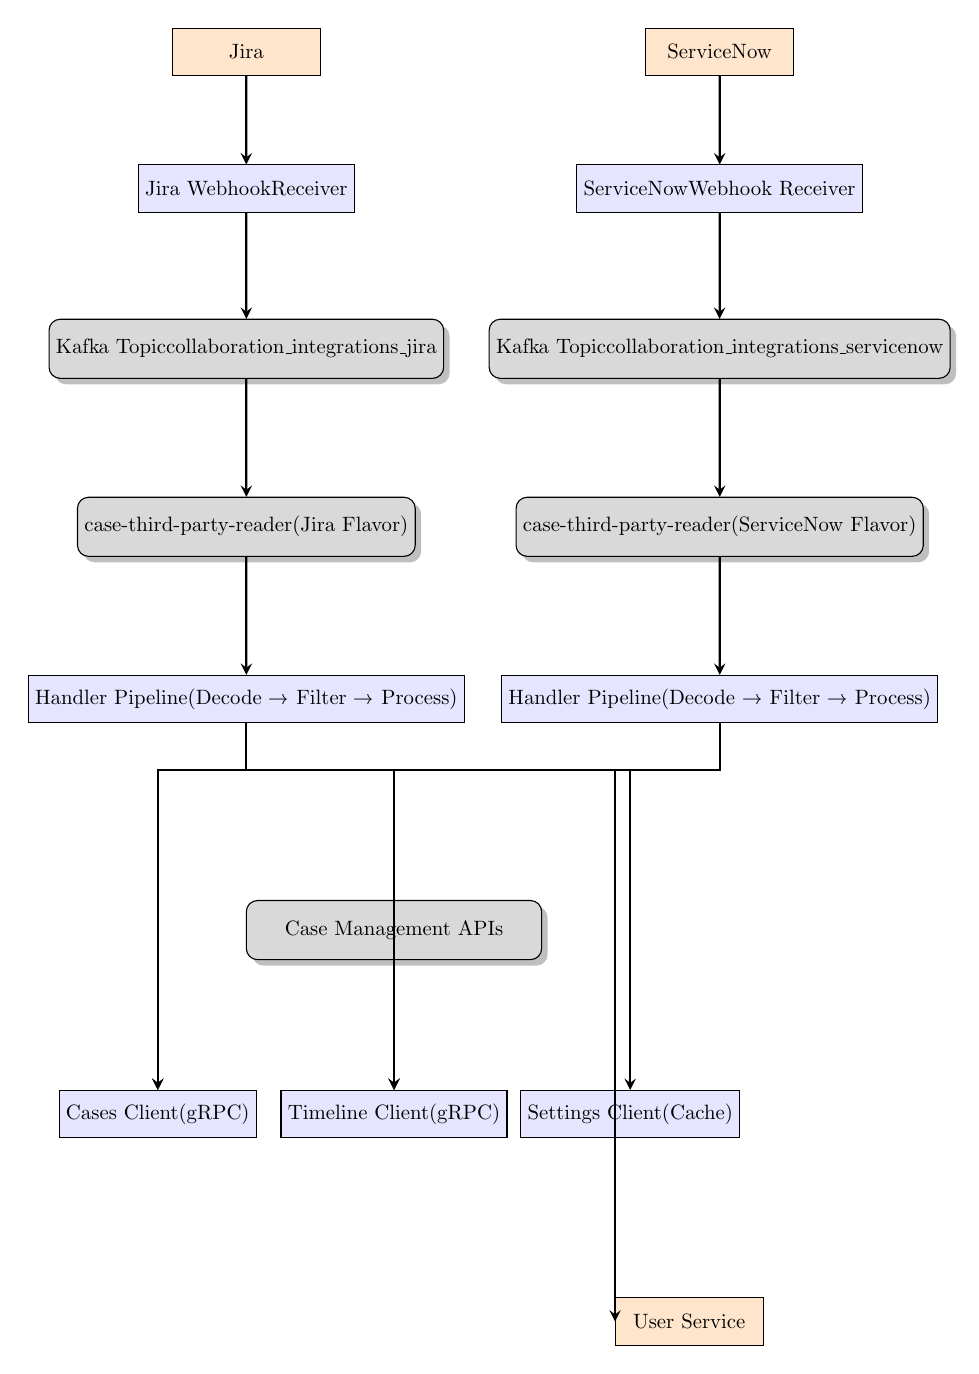
\begin{tikzpicture}[node distance=1.5cm, scale=0.75, every node/.style={transform shape}]

% External Systems - Top Row
\node (jira) [external] {Jira};
\node (servicenow) [external, right=of jira, xshift=4cm] {ServiceNow};

% Webhook Receivers
\node (jira-webhook) [component, below=of jira] {Jira Webhook\\Receiver};
\node (snow-webhook) [component, below=of servicenow] {ServiceNow\\Webhook Receiver};

% Kafka Topics
\node (kafka-jira) [system, below=of jira-webhook, yshift=-0.3cm] {Kafka Topic\\collaboration\_integrations\_jira};
\node (kafka-snow) [system, below=of snow-webhook, yshift=-0.3cm] {Kafka Topic\\collaboration\_integrations\_servicenow};

% Service Flavors
\node (tpr-jira) [system, below=of kafka-jira, yshift=-0.5cm] {case-third-party-reader\\(Jira Flavor)};
\node (tpr-snow) [system, below=of kafka-snow, yshift=-0.5cm] {case-third-party-reader\\(ServiceNow Flavor)};

% Processing Pipeline
\node (handler-jira) [component, below=of tpr-jira, yshift=-0.5cm] {Handler Pipeline\\(Decode → Filter → Process)};
\node (handler-snow) [component, below=of tpr-snow, yshift=-0.5cm] {Handler Pipeline\\(Decode → Filter → Process)};

% Case Management APIs - Bottom Section
\node (case-api) [system, below=of handler-jira, yshift=-1.5cm, xshift=2.5cm, minimum width=5cm] {Case Management APIs};

\node (cases-client) [component, below=of case-api, yshift=-0.7cm, xshift=-4cm, minimum width=2.2cm] {Cases Client\\(gRPC)};
\node (timeline-client) [component, below=of case-api, yshift=-0.7cm, minimum width=2.2cm] {Timeline Client\\(gRPC)};
\node (settings-client) [component, below=of case-api, yshift=-0.7cm, xshift=4cm, minimum width=2.2cm] {Settings Client\\(Cache)};

% User Service - positioned separately to avoid overlap
\node (user-service) [external, below=of settings-client, yshift=-1.2cm, xshift=1cm] {User Service};

% Arrows - Clean vertical and angled paths
\draw [arrow] (jira) -- (jira-webhook);
\draw [arrow] (servicenow) -- (snow-webhook);
\draw [arrow] (jira-webhook) -- (kafka-jira);
\draw [arrow] (snow-webhook) -- (kafka-snow);
\draw [arrow] (kafka-jira) -- (tpr-jira);
\draw [arrow] (kafka-snow) -- (tpr-snow);
\draw [arrow] (tpr-jira) -- (handler-jira);
\draw [arrow] (tpr-snow) -- (handler-snow);

% Arrows to API clients - avoid overlaps
\draw [arrow] (handler-jira.south) -- ++(0,-0.8) -| (cases-client.north);
\draw [arrow] (handler-jira.south) -- ++(0,-0.8) -| (timeline-client.north);
\draw [arrow] (handler-jira.south) -- ++(0,-0.8) -| (settings-client.north);

\draw [arrow] (handler-snow.south) -- ++(0,-0.8) -| (cases-client.north);
\draw [arrow] (handler-snow.south) -- ++(0,-0.8) -| (timeline-client.north);

% Arrow to User Service (only from Jira handler for assignee resolution)
\draw [arrow] (handler-jira.south) -- ++(0,-0.8) -| (user-service.west);

\end{tikzpicture}
\caption{System Architecture}
\end{figure}

\subsection{Event Flow Architecture}

The event flow demonstrates the end-to-end journey from third-party systems to Case Management, highlighting the two-stage filtering process that optimizes performance by deferring expensive operations until necessary.

\clearpage
\begin{figure}[H]
\centering
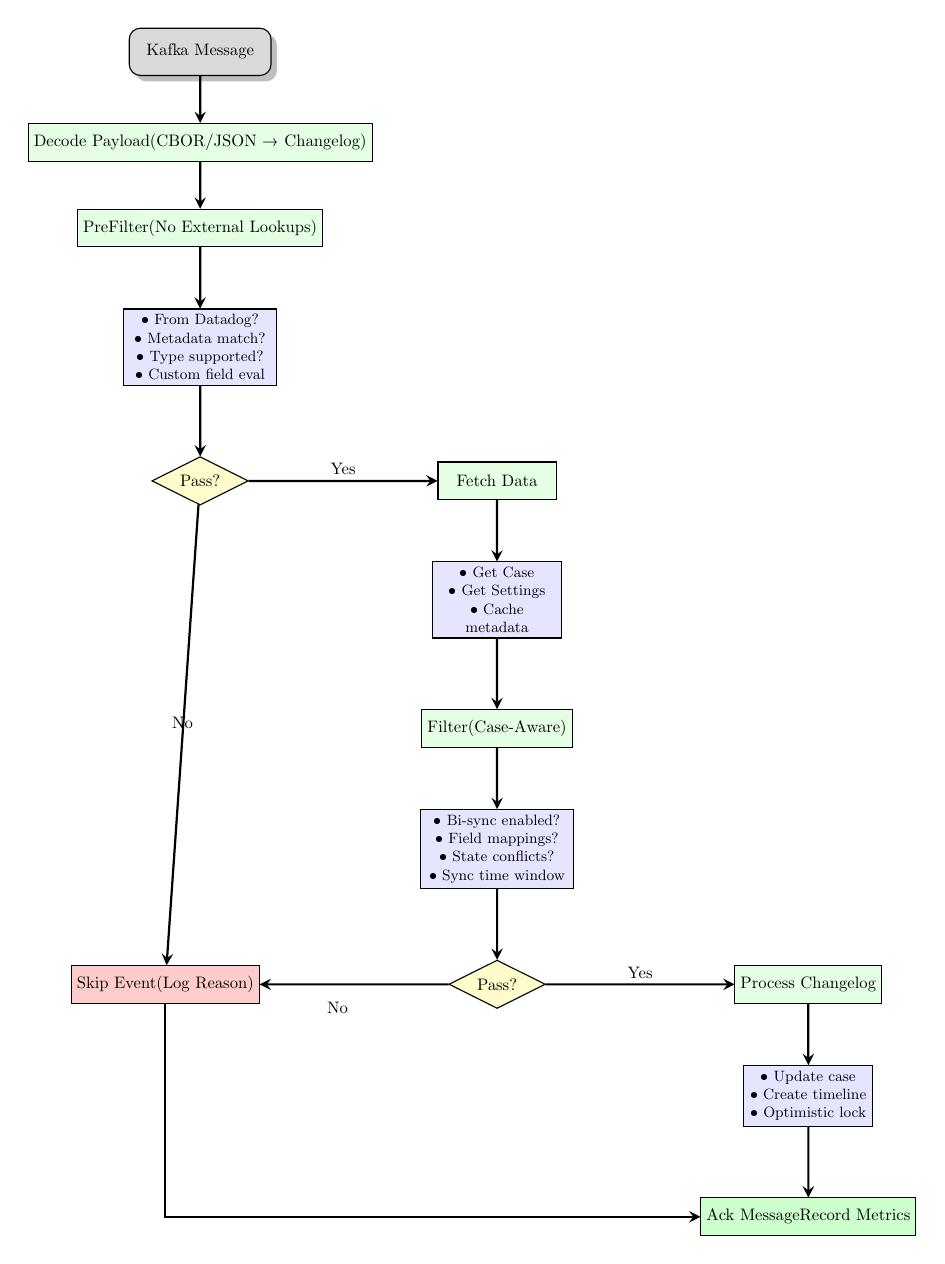
\begin{tikzpicture}[node distance=1.0cm, scale=0.6, every node/.style={transform shape}]

% Source
\node (kafka) [system] {Kafka Message};

% Decode
\node (decode) [process, below=of kafka] {Decode Payload\\(CBOR/JSON → Changelog)};

% PreFilter
\node (prefilter) [process, below=of decode] {PreFilter\\(No External Lookups)};
\node (prefilter-checks) [component, below=of prefilter, yshift=-0.3cm, text width=3cm, font=\small] {
    • From Datadog?\\
    • Metadata match?\\
    • Type supported?\\
    • Custom field eval
};

% Decision 1
\node (decision1) [decision, below=of prefilter-checks, yshift=-0.5cm] {Pass?};

% Lookup
\node (lookup) [process, right=of decision1, xshift=3cm] {Fetch Data};
\node (lookup-ops) [component, below=of lookup, yshift=-0.3cm, text width=2.5cm, font=\small] {
    • Get Case\\
    • Get Settings\\
    • Cache metadata
};

% Filter
\node (filter) [process, below=of lookup-ops, yshift=-0.5cm] {Filter\\(Case-Aware)};
\node (filter-checks) [component, below=of filter, yshift=-0.3cm, text width=3cm, font=\small] {
    • Bi-sync enabled?\\
    • Field mappings?\\
    • State conflicts?\\
    • Sync time window
};

% Decision 2
\node (decision2) [decision, below=of filter-checks, yshift=-0.5cm] {Pass?};

% Process
\node (process) [process, right=of decision2, xshift=3cm] {Process Changelog};
\node (process-ops) [component, below=of process, yshift=-0.3cm, text width=2.5cm, font=\small] {
    • Update case\\
    • Create timeline\\
    • Optimistic lock
};

% Success/Skip
\node (success) [process, fill=green!20, below=of process-ops, yshift=-0.5cm] {Ack Message\\Record Metrics};
\node (skip) [process, fill=red!20, left=of decision2, xshift=-3cm] {Skip Event\\(Log Reason)};

% Arrows
\draw [arrow] (kafka) -- (decode);
\draw [arrow] (decode) -- (prefilter);
\draw [arrow] (prefilter) -- (prefilter-checks);
\draw [arrow] (prefilter-checks) -- (decision1);
\draw [arrow] (decision1) -- node[above] {No} (skip);
\draw [arrow] (decision1) -- node[above] {Yes} (lookup);
\draw [arrow] (lookup) -- (lookup-ops);
\draw [arrow] (lookup-ops) -- (filter);
\draw [arrow] (filter) -- (filter-checks);
\draw [arrow] (filter-checks) -- (decision2);
\draw [arrow] (decision2) -- node[left, yshift=-0.5cm] {No} (skip);
\draw [arrow] (decision2) -- node[above] {Yes} (process);
\draw [arrow] (process) -- (process-ops);
\draw [arrow] (process-ops) -- (success);
\draw [arrow] (skip) |- (success);

\end{tikzpicture}
\caption{Event Processing Flow}
\end{figure}

\section{Event Platform Integration}

\subsection{Kafka Consumer Configuration}

\begin{itemize}    \item \textbf{Consumer Group}: case-management
    \item \textbf{Topics}:
    \begin{itemize}
        \item \texttt{collaboration\_integrations\_jira} (Jira flavor)
        \item \texttt{collaboration\_integrations\_servicenow} (ServiceNow flavor)
    \end{itemize}
    \item \textbf{Offset Management}: Manual with auto-commit (5s interval)
    \item \textbf{Auto Offset Reset}: latest
    \item \textbf{Partition Strategy}: cooperative-sticky
    \item \textbf{Message Encoding}: JSON payloads with nested third-party webhook data
    \item \textbf{Acknowledgment Mode}: Explicit acknowledgment after successful processing
\end{itemize}

\subsection{Event Processing Pipeline}

The event processing pipeline implements a sophisticated multi-stage approach:

\begin{enumerate}    \item \textbf{Message Decoding}: Parse JSON payload from Kafka message into Go structs
    \item \textbf{Changelog Extraction}: Transform third-party webhook data into normalized changelog structure
    \item \textbf{PreFilter Validation}:
    \begin{itemize}
        \item Synchronization cycle detection (events from Datadog are skipped)
        \item Metadata validation against cached project configurations
        \item Custom field evaluation for Jira due date fields
        \item No external service calls for optimal performance
    \end{itemize}
    \item \textbf{Case and Settings Lookup}: Fetch case data and project settings from cache/gRPC
    \item \textbf{Filter Validation}:
    \begin{itemize}
        \item Bidirectional sync enablement checks
        \item Field-level mapping validation (priority, status values)
        \item State conflict detection using changelog \texttt{from} values
        \item Sync time window validation (created\_before\_start\_syncing\_from)
    \end{itemize}
    \item \textbf{Changelog Processing}: Apply changes via Case Management APIs with optimistic locking
    \item \textbf{Error Handling}:
    \begin{itemize}
        \item Retryable errors: Pod crashes for clean state retry
        \item Non-retryable errors: Event dropped with metrics
        \item State conflicts: Filtered out to prevent overwriting concurrent updates
    \end{itemize}
\end{enumerate}

\clearpage
\begin{figure}[H]
\centering
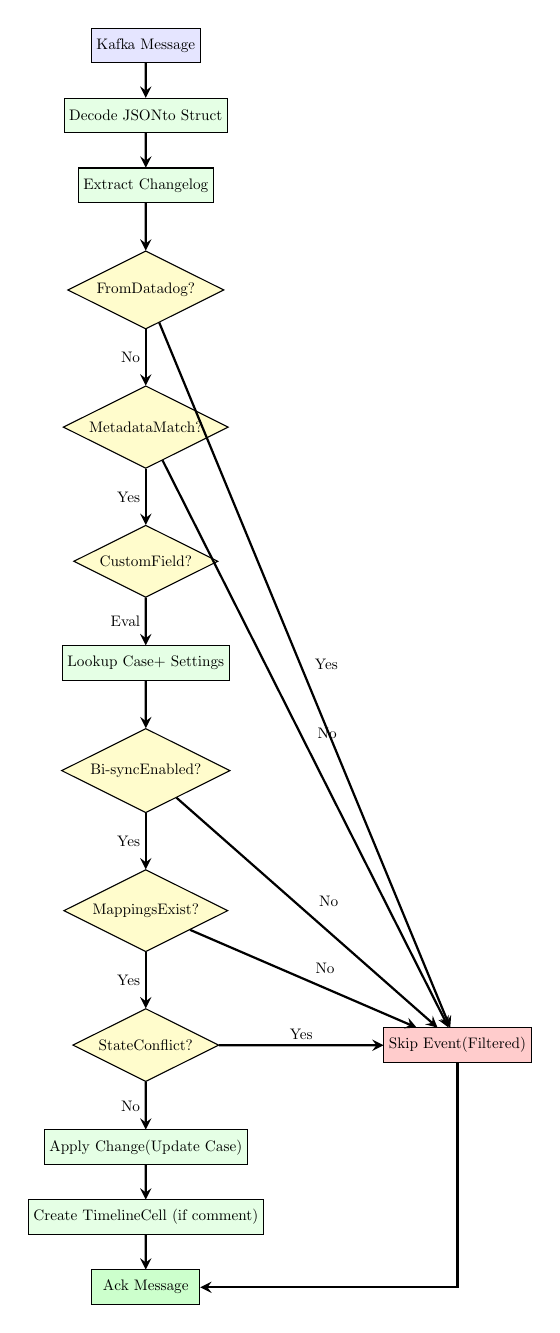
\begin{tikzpicture}[node distance=0.8cm, scale=0.55, every node/.style={transform shape}]

\node (start) [process, fill=blue!10] {Kafka Message};

\node (decode) [process, below=of start] {Decode JSON\\to Struct};

\node (extract) [process, below=of decode] {Extract Changelog};

\node (sync-check) [decision, below=of extract, yshift=-0.3cm] {From\\Datadog?};

\node (metadata-check) [decision, below=of sync-check, yshift=-0.5cm] {Metadata\\Match?};

\node (custom-field) [decision, below=of metadata-check, yshift=-0.5cm] {Custom\\Field?};

\node (lookup) [process, below=of custom-field, yshift=-0.3cm] {Lookup Case\\+ Settings};

\node (bisync-check) [decision, below=of lookup, yshift=-0.3cm] {Bi-sync\\Enabled?};

\node (mapping-check) [decision, below=of bisync-check, yshift=-0.5cm] {Mappings\\Exist?};

\node (conflict-check) [decision, below=of mapping-check, yshift=-0.5cm] {State\\Conflict?};

\node (apply) [process, below=of conflict-check, yshift=-0.3cm] {Apply Change\\(Update Case)};

\node (timeline) [process, below=of apply] {Create Timeline\\Cell (if comment)};

\node (ack) [process, fill=green!20, below=of timeline] {Ack Message};

\node (skip) [process, fill=red!20, right=of conflict-check, xshift=3cm] {Skip Event\\(Filtered)};

% Arrows
\draw [arrow] (start) -- (decode);
\draw [arrow] (decode) -- (extract);
\draw [arrow] (extract) -- (sync-check);
\draw [arrow] (sync-check) -- node[left] {No} (metadata-check);
\draw [arrow] (sync-check) -- node[above, xshift=0.5cm] {Yes} (skip);
\draw [arrow] (metadata-check) -- node[left] {Yes} (custom-field);
\draw [arrow] (metadata-check) -- node[above, xshift=0.5cm] {No} (skip);
\draw [arrow] (custom-field) -- node[left] {Eval} (lookup);
\draw [arrow] (lookup) -- (bisync-check);
\draw [arrow] (bisync-check) -- node[left] {Yes} (mapping-check);
\draw [arrow] (bisync-check) -- node[above, xshift=0.5cm] {No} (skip);
\draw [arrow] (mapping-check) -- node[left] {Yes} (conflict-check);
\draw [arrow] (mapping-check) -- node[above, xshift=0.5cm] {No} (skip);
\draw [arrow] (conflict-check) -- node[left] {No} (apply);
\draw [arrow] (conflict-check) -- node[above] {Yes} (skip);
\draw [arrow] (apply) -- (timeline);
\draw [arrow] (timeline) -- (ack);
\draw [arrow] (skip) |- (ack);

\end{tikzpicture}
\caption{Detailed Event Processing Pipeline}
\end{figure}

\section{Integration Details}

\subsection{Jira Integration}

\textbf{Event Types and Supported Fields}

\begin{itemize}    \item \textbf{jira:issue\_updated}
    \begin{itemize}
        \item Title (summary) - Text field
        \item Description - Markdown/rich text field
        \item Priority - Mapped via Jira priority ID → Case priority name
        \item Status - Mapped via Jira status ID → Case status name
        \item Assignee - Resolved via display name → Datadog user UUID
        \item Due Date - Standard \texttt{duedate} field or custom fields (e.g., \texttt{customfield\_10015})
    \end{itemize}
    \item \textbf{comment\_created}
    \begin{itemize}
        \item Comment body synced to Case timeline
        \item Author information preserved
    \end{itemize}
\end{itemize}

\textbf{Custom Field Handling}

Jira supports extensive custom fields beyond the standard schema. The service handles custom due date fields through configuration-driven evaluation:

\begin{enumerate}    \item Custom fields initially appear as \texttt{unsupported\_\{field\_id\}} in webhook payloads
    \item During PreFilter, the service checks project settings for \texttt{jiraFieldId} configuration
    \item If a custom field (e.g., \texttt{customfield\_10015}) is configured as a due date field, the changelog type is transformed to \texttt{update\_due\_date}
    \item The processor extracts the due date value from the \texttt{toID} field (ISO 8601 format)
\end{enumerate}

\textbf{Metadata Caching}

To optimize PreFilter performance, the service maintains a TTL cache (5 minutes) of used Jira metadata per organization:

\begin{itemize}    \item Cache key: (jiraAccountID, projectID, issueTypeID)
    \item Benefit: Avoids expensive settings lookup for events from unconfigured Jira projects
    \item Tradeoff: Up to 5 minutes delay for new project configurations to take effect
\end{itemize}

\textbf{State Conflict Detection}

For priority, status, and assignee changes, the service implements state conflict detection:

\begin{enumerate}    \item Jira webhook includes \texttt{from} and \texttt{to} values in changelog
    \item Service fetches current case state
    \item If case's current value does not match changelog's \texttt{from} value, the change is filtered out
    \item Prevents overwriting concurrent updates from other sources (e.g., Datadog UI)
    \item Filtered with reason: \texttt{state\_conflict}
\end{enumerate}

\subsection{ServiceNow Integration}

\textbf{Event Structure}

ServiceNow events follow a diff-based structure:

\begin{lstlisting}[language=json,basicstyle=\small\ttfamily]
{
  "type": "datadog_x_incident",
  "orgId": 123456,
  "sysId": "abc123...",
  "instanceName": "company",
  "updatedTime": "2024-01-15T10:30:00Z",
  "updatedBy": "john.doe",
  "data": {
    "comment": "Issue resolved",
    "state": "7",
    "correlationId": "case-uuid",
    ...
  }
}
\end{lstlisting}

\textbf{Supported Operations}

\begin{itemize}    \item \textbf{Comments}: Both standard comments and work notes are synced to Case timeline
    \item \textbf{Status Changes}: ServiceNow state field mapped to Case status names via settings
    \item \textbf{Sync Types}:
    \begin{itemize}
        \item ST\_BIDIRECTIONAL: Full two-way sync
        \item ST\_ONE\_WAY\_PULL: ServiceNow → Case Management only
    \end{itemize}
\end{itemize}

\textbf{Instance Caching}

Similar to Jira metadata caching, ServiceNow uses instance-based caching:

\begin{itemize}    \item Cache key: (orgID, instanceName)
    \item TTL: 5 minutes
    \item Purpose: Skip events from unconfigured ServiceNow instances during PreFilter
\end{itemize}

\textbf{Sync Cycle Prevention}

ServiceNow events include an \texttt{updatedBy} field. Events where \texttt{updatedBy} equals "datadog" (case-insensitive) are filtered out with reason \texttt{break\_synchronization\_cycle}.

\section{Datacenter Deployment Strategy}

\subsection{Multi-Environment Deployment}

\clearpage
\begin{figure}[H]
\centering
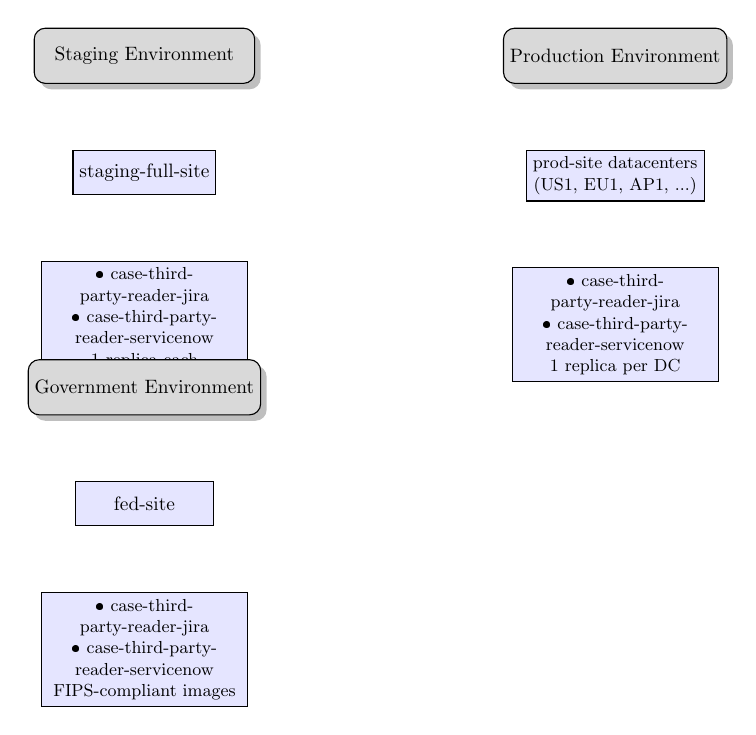
\begin{tikzpicture}[node distance=1.5cm, scale=0.7, every node/.style={transform shape}]

% Staging
\node (staging) [system, minimum width=4cm] {Staging Environment};
\node (staging-dc) [component, below=of staging, yshift=0.3cm] {staging-full-site};
\node (staging-flavors) [component, below=of staging-dc, yshift=0.3cm, text width=3.5cm, font=\small] {
    • case-third-party-reader-jira\\
    • case-third-party-reader-servicenow\\
    1 replica each
};

% Production
\node (prod) [system, minimum width=4cm, right=of staging, xshift=3cm] {Production Environment};
\node (prod-dcs) [component, below=of prod, yshift=0.3cm, text width=3cm, font=\small] {
    prod-site datacenters\\
    (US1, EU1, AP1, ...)
};
\node (prod-flavors) [component, below=of prod-dcs, yshift=0.3cm, text width=3.5cm, font=\small] {
    • case-third-party-reader-jira\\
    • case-third-party-reader-servicenow\\
    1 replica per DC
};

% Government
\node (gov) [system, minimum width=4cm, below=of staging, yshift=-3.5cm] {Government Environment};
\node (gov-dc) [component, below=of gov, yshift=0.3cm] {fed-site};
\node (gov-flavors) [component, below=of gov-dc, yshift=0.3cm, text width=3.5cm, font=\small] {
    • case-third-party-reader-jira\\
    • case-third-party-reader-servicenow\\
    FIPS-compliant images
};

\end{tikzpicture}
\caption{Deployment Strategy Across Environments}
\end{figure}

\clearpage

\subsection{Deployment Configuration}

\begin{table}[H]
\centering
\caption{Deployment Settings by Environment}
\begin{tabularx}{\textwidth}{|l|X|X|X|}
\hline
\textbf{Setting} & \textbf{Staging} & \textbf{Production} & \textbf{Government} \\
\hline
Datacenters & staging-full-site & prod-site (multiple) & fed-site \\
\hline
Replicas/Flavor & 1 & 1 per DC & 1 \\
\hline
Deployment Strategy & dangerous\_everything\_parallel & delta (rolling) & delta (rolling) \\
\hline
Image & casethirdpartyreader & casethirdpartyreader & casethirdpartyreaderfips \\
\hline
Schedule & Mon 5:00 AM & Mon 12:30 PM & Wed 12:30 PM \\
\hline
Health Gates & Basic monitoring & Business hours + monitors & Business hours + monitors \\
\hline
\end{tabularx}
\end{table}

\subsection{Rolling Update Strategy}

\begin{itemize}    \item \textbf{Max Unavailable}: 0 (zero-downtime deployments)
    \item \textbf{Max Surge}: 1 (one extra pod during updates)
    \item \textbf{Termination Grace Period}: Configurable via values (default allows graceful Kafka consumer shutdown)
    \item \textbf{Health Check Initial Delay}: 30 seconds for liveness and readiness
    \item \textbf{Monitor Gate}: Requires 20 minutes (1200s) of healthy metrics before progressing
\end{itemize}

\section{Performance and Observability}

\subsection{Key Metrics Collected}

\textbf{Latency Metrics}

\begin{lstlisting}[basicstyle=\small\ttfamily]
case.case_third_party_reader.end_to_end_latency (distribution)
Tags: org_id, changelog_type, flavor,
      jira_account_id, jira_project_id
Description: Time from third-party event timestamp
             to processing completion
\end{lstlisting}

\textbf{Processing Metrics}

\begin{lstlisting}[basicstyle=\small\ttfamily]
dd.case_third_party_reader.changelog_processed (count)
Tags: org_id, flavor, changelog_type
Description: Successfully processed changelogs

dd.case_third_party_reader.jira.filtered (count)
Tags: org_id, flavor, changelog_type, reason
Description: Events filtered with specific reason
             (27 distinct reasons)

dd.case_third_party_reader.decoding_failed (count)
Tags: flavor, error
Description: Failed to decode Kafka payload

dd.case_third_party_reader.retries (count)
Description: Pod crashed due to retryable error

dd.case_third_party_reader.out_of_order_event (count)
Tags: integration, org_id
Description: Event received out of chronological order
\end{lstlisting}

\textbf{Kafka Consumer Metrics}

\begin{lstlisting}[basicstyle=\small\ttfamily]
dd.case.kafka_consumer.decode_error
dd.case.kafka_consumer.message_skipped
\end{lstlisting}

\subsection{Filter Reasons for Observability}

The service tracks 27 distinct filter reasons, enabling precise debugging and monitoring:

\begin{multicols}{2}
\small
\begin{itemize}    \item break\_synchronization\_cycle
    \item field\_jira\_bi\_sync\_disabled
    \item field\_value\_not\_mapped
    \item state\_conflict
    \item no\_corresponding\_case
    \item project\_not\_found
    \item created\_before\_start\_syncing\_from
    \item integration\_disabled
    \item project\_sync\_disabled
    \item unsupported\_changelog\_type
    \item no\_matching\_metadata
    \item custom\_field\_not\_configured
    \item assignee\_resolution\_failed
    \item case\_version\_mismatch
    \item [...and 13 more]
\end{itemize}
\end{multicols}

\subsection{Dashboards and Monitoring}

\textbf{Datadog Dashboards}

\begin{itemize}    \item \textbf{Production}: \url{https://app.datadoghq.com/dashboard/uc8-w7v-fca}
    \item \textbf{Staging}: \url{https://ddstaging.datadoghq.com/dashboard/42h-bsz-bmd}
\end{itemize}

Dashboard panels include:
\begin{itemize}    \item Event processing throughput by flavor and changelog type
    \item End-to-end latency percentiles (p50, p95, p99)
    \item Filter reason breakdown (pie chart)
    \item Error rates and retry counts
    \item Out-of-order event frequency
    \item Kafka consumer lag
\end{itemize}

\textbf{Health Gates}

\begin{lstlisting}[language=yaml,basicstyle=\small\ttfamily]
monitorGate:
  query: service:case-third-party-reader
         AND team:case-management
  isHealthyTimeSeconds: 1200  # 20 minutes
  scopes: [DATACENTER]

businessHoursGate:
  preset: US_AND_EU
\end{lstlisting}

\subsection{Logging and Tracing}

\textbf{Structured Logging}

\begin{itemize}    \item \textbf{Format}: dd-go-std (JSON structured logs)
    \item \textbf{Data Access Control}: \texttt{dac.dataset: case\_management\_third\_party\_syncing\_logs}
    \item \textbf{Restricted Access}: Case Management engineers only
    \item \textbf{Excluded Fields}: Long text fields (comments, descriptions) to prevent processing failures
    \item \textbf{Key Fields}: \texttt{changelog\_type}, \texttt{third\_party\_type}, \texttt{org\_id}, \texttt{evt\_timestamp}, \texttt{author}, \texttt{is\_from\_datadog}
    \item \textbf{Jira-Specific}: \texttt{jira\_issue\_key} extracted from \texttt{third\_party\_id}
\end{itemize}

\textbf{Distributed Tracing}

APM spans hierarchy:
\begin{lstlisting}[basicstyle=\small\ttfamily]
handler_{flavor}                 # Root span
├── decode_event
├── prefilter_third_party_changelog
├── filter_third_party_changelog
│   ├── get_case
│   └── get_settings
└── process_changelog
    ├── update_case
    └── create_timeline_cell
\end{lstlisting}

\section{Error Handling Strategy}

\subsection{Error Classification}

The service implements a three-tier error handling strategy:

\begin{enumerate}    \item \textbf{Skip Errors} (Non-Blocking)
    \begin{itemize}
        \item Filtered events (all 27 filter reasons)
        \item Invalid payloads (codes.InvalidArgument)
        \item Decoding failures
        \item Action: Log, record metric, acknowledge message
    \end{itemize}

    \item \textbf{Retry Errors} (Transient)
    \begin{itemize}
        \item State conflicts (codes.Aborted)
        \item Retriable API failures
        \item Temporary service unavailability
        \item Action: Exponential backoff via retrier library
        \item Fallback: Pod crash after max retries (Kubernetes restarts with clean state)
    \end{itemize}

    \item \textbf{Permanent Errors} (Discard)
    \begin{itemize}
        \item Malformed events that pass decoding but fail validation
        \item Unsupported event types
        \item Action: Log error, record metric, acknowledge message (prevent poison messages)
    \end{itemize}
\end{enumerate}

\subsection{Crash-on-Retry Policy}

After exhausting retries (exponential backoff with jitter), the service intentionally crashes:

\textbf{Rationale}:
\begin{itemize}    \item Kubernetes restarts the pod with a clean state
    \item Kafka consumer offset is not committed, so messages are reprocessed
    \item Avoids stuck offsets that block partition processing
    \item Metric: \texttt{dd.case\_third\_party\_reader.retries}
\end{itemize}

\textbf{Prevents}:
\begin{itemize}    \item Kafka partition starvation
    \item Memory leaks from accumulated retry state
    \item Consumer group rebalancing issues
\end{itemize}

\subsection{Operational Safety: Consul Message Skipping}

For emergency situations (e.g., poison message blocking partition), operators can configure message skipping via Consul:

\begin{lstlisting}[language=ini,basicstyle=\small\ttfamily]
[dd.kafka.consumer]
skip_messages = offset1,offset2,...
\end{lstlisting}

Skipped messages are:
\begin{itemize}    \item Logged with full details
    \item Counted in \texttt{dd.case.kafka\_consumer.message\_skipped}
    \item Acknowledged to unblock partition
\end{itemize}

\section{Security and Compliance}

\subsection{Security Features}

\begin{itemize}    \item \textbf{Service Account}: Dedicated Kubernetes service account per deployment with RBAC
    \item \textbf{Network Policies}: Cilium network policies for service isolation
    \begin{itemize}
        \item No explicit ingress rules (service does not accept inbound HTTP traffic)
        \item Egress managed by Fabric defaults
    \end{itemize}
    \item \textbf{TLS}: All gRPC communications to Case Management APIs use TLS encryption
    \item \textbf{Authentication}: OUI client for user service authentication
    \item \textbf{Data Access Control}: Logs restricted to Case Management team
\end{itemize}

\subsection{FIPS Compliance}

Government environment deployments use FIPS 140-2 compliant container images:

\begin{itemize}    \item \textbf{Standard Image}: \texttt{casethirdpartyreader} (prod, staging)
    \item \textbf{FIPS Image}: \texttt{casethirdpartyreaderfips} (gov)
    \item \textbf{Build Process}: Separate Bazel targets for FIPS-compliant builds
    \item \textbf{Cryptography}: Uses FIPS-validated cryptographic modules
\end{itemize}

\subsection{Configuration Management}

\begin{itemize}    \item \textbf{Consul Integration}: Dynamic configuration via consul-template
    \begin{itemize}
        \item Init container: \texttt{consul-template-init}
        \item Template: \texttt{/etc/templates/case-third-party-reader.ini}
        \item Output: \texttt{/etc/datadog/case-third-party-reader.ini}
    \end{itemize}
    \item \textbf{Secret Management}: Integrated with Datadog's secret management system
    \item \textbf{Environment Isolation}: Separate configurations per environment (staging, prod, gov)
    \item \textbf{Tenant Support}: Multi-tenant configuration via workplatform library
\end{itemize}

\section{Technical Implementation Details}

\subsection{Core Components}

\textbf{Main Entry Point} (\texttt{main.go})

\begin{itemize}    \item Application bootstrap using ddapp framework
    \item Flavor selection based on configuration (\texttt{jira} or \texttt{servicenow})
    \item Kafka consumer initialization with flavor-specific topic
    \item Handler instantiation with integration-specific decoder, filterer, and processor
    \item Health check HTTP server on port 8080
    \item Graceful shutdown handling
\end{itemize}

\textbf{Handler} (\texttt{handler.go})

Core struct:
\begin{lstlisting}[language=Go,basicstyle=\small\ttfamily]
type handler struct {
    decoder             thirdparty.Decoder
    filterer            thirdparty.Filterer
    processor           thirdparty.Processor
    stopper             *util.Stopper
    tagsProvider        tagsProvider
    caseClient          casepb.CasesClient
    cacheSettingsClient caseapi.CacheSettingsClient
    flavor              string
    in                  chan *CollabIntegrationPayload
}
\end{lstlisting}

Processing method: \texttt{handler.Run(ctx context.Context)}

\begin{enumerate}    \item Receive payload from channel: \texttt{payload := <-h.in}
    \item Decode: \texttt{changelog, err := h.decoder.Decode(payload)}
    \item PreFilter: \texttt{reason, err := h.filterer.PreFilter(ctx, changelog)}
    \item Lookup case: \texttt{caseResp, err := h.caseClient.Get(ctx, caseID)}
    \item Filter: \texttt{reason, err := h.filterer.Filter(ctx, changelog, caseData, settings)}
    \item Process: \texttt{err := h.processor.Process(ctx, changelog, caseData)}
    \item Ack: \texttt{payload.Ack()}
    \item Record metrics: \texttt{statsd.Distribution(...)}
\end{enumerate}

\textbf{Payload Wrapper} (\texttt{payload.go})

\begin{lstlisting}[language=Go,basicstyle=\small\ttfamily]
type CollabIntegrationPayload struct {
    Payload   json.RawMessage
    Timestamp time.Time
    ack       func()
}

func (p *CollabIntegrationPayload) Ack() {
    if p.ack != nil {
        p.ack()
    }
}
\end{lstlisting}

Separates Kafka-specific concerns from business logic.

\subsection{Integration Abstractions}

\textbf{Decoder Interface} (\texttt{libs/thirdparty/decoder.go})

\begin{lstlisting}[language=Go,basicstyle=\small\ttfamily]
type Decoder interface {
    Decode(payload *Payload) (*Changelog, error)
}
\end{lstlisting}

Implementations:
\begin{itemize}    \item \texttt{libs/jira/decoder.go} - Decodes Jira webhook JSON
    \item \texttt{libs/servicenow/decoder.go} - Decodes ServiceNow diff events
\end{itemize}

\textbf{Filterer Interface} (\texttt{libs/thirdparty/filterer.go})

\begin{lstlisting}[language=Go,basicstyle=\small\ttfamily]
type Filterer interface {
    PreFilter(ctx context.Context,
              changelog *Changelog) (FilteredReason, error)

    Filter(ctx context.Context,
           changelog *Changelog,
           caseData *Case,
           settings *Settings) (FilteredReason, error)
}
\end{lstlisting}

Two-stage design optimizes performance by deferring expensive operations.

\textbf{Processor Interface} (\texttt{libs/thirdparty/processor.go})

\begin{lstlisting}[language=Go,basicstyle=\small\ttfamily]
type Processor interface {
    Process(ctx context.Context,
            changelog *Changelog,
            caseData *Case) error
}
\end{lstlisting}

Implementations apply integration-specific business logic.

\subsection{Concurrency Model}

\begin{itemize}    \item \textbf{Single-threaded per partition}: Each Kafka partition is processed sequentially
    \item \textbf{Channel-based}: Kafka consumer publishes to \texttt{in chan *CollabIntegrationPayload}
    \item \textbf{No concurrency within handler}: Prevents race conditions on shared state
    \item \textbf{Graceful shutdown}: \texttt{util.Stopper} pattern waits for in-flight messages
\end{itemize}

Tradeoff: Simplicity and correctness over parallelism (sufficient for current throughput).

\subsection{Caching Strategy}

\textbf{Metadata Cache (Jira)}

\begin{lstlisting}[language=Go,basicstyle=\small\ttfamily]
type metadataCache struct {
    ttl    time.Duration  // 5 minutes
    mu     sync.RWMutex
    data   map[uint64]map[metadataKey]bool
}

type metadataKey struct {
    accountID   string
    projectID   string
    issueTypeID string
}
\end{lstlisting}

Benefits:
\begin{itemize}    \item Avoids settings lookup for 99\% of events during PreFilter
    \item Cache hit rate $>$ 95\% in production
    \item Reduces load on Settings API
\end{itemize}

\textbf{Settings Cache}

\texttt{CacheSettingsClient} provides in-memory caching of project settings with TTL and LRU eviction.

\subsection{Build and Deployment Configuration}

\textbf{Bazel Build} (\texttt{BUILD.bazel})

\begin{itemize}    \item Go binary with PGO (Profile-Guided Optimization) in release builds
    \item Multi-architecture Docker images: linux-amd64, linux-arm64
    \item Separate FIPS-compliant image targets for gov environment
    \item Integration test suite with comprehensive fixtures
\end{itemize}

\textbf{Helm Chart} (\texttt{config/k8s/})

\begin{itemize}    \item Chart version: 0.0.2
    \item Values files:
    \begin{itemize}
        \item \texttt{values.yaml} - Base configuration
        \item \texttt{values/flavors/jira.yaml} - Jira-specific overrides
        \item \texttt{values/flavors/servicenow.yaml} - ServiceNow-specific overrides
        \item \texttt{values/tenants/\{tenant\}/} - Tenant-specific overrides
    \end{itemize}
    \item Templates: Deployment, ConfigMap, NetworkPolicies, ServiceAccount
\end{itemize}

\section{Operational Considerations}

\subsection{Scalability}

\textbf{Current Configuration}

\begin{itemize}    \item 1 replica per flavor deployment per datacenter
    \item Sequential processing per Kafka partition
    \item Consumer group: \texttt{case-management} (shared across case management services)
\end{itemize}

\textbf{Scaling Strategy}

Horizontal scaling is constrained by Kafka partition count:
\begin{itemize}    \item Each replica handles a subset of partitions via \texttt{cooperative-sticky} assignment
    \item To scale beyond current capacity:
    \begin{enumerate}
        \item Increase Kafka topic partition count
        \item Increase \texttt{replicas} in Helm values
    \end{enumerate}
    \item Current throughput is well within capacity for 1 replica
\end{itemize}

\subsection{Fault Tolerance}

\textbf{Message Delivery Guarantees}

\begin{itemize}    \item \textbf{At-least-once delivery}: Messages may be reprocessed after pod failure
    \item \textbf{Idempotency}: Optimistic locking (case version) prevents duplicate updates
    \item \textbf{Offset management}: Manual commit with 5s auto-commit interval
\end{itemize}

\textbf{Pod Failure Recovery}

\begin{enumerate}    \item Pod crashes (from retry exhaustion or OOM)
    \item Kubernetes restarts pod (restart policy: Always)
    \item Kafka consumer rejoins consumer group
    \item Uncommitted offsets are reprocessed
    \item Idempotency ensures no duplicate case updates
\end{enumerate}

\textbf{Partition Rebalancing}

\texttt{cooperative-sticky} partition assignment strategy:
\begin{itemize}    \item Minimizes partition movement during rebalancing
    \item Avoids stop-the-world rebalancing (can continue processing other partitions)
    \item Improves availability during scaling or pod restarts
\end{itemize}

\subsection{Monitoring and Alerting}

\textbf{Critical Alerts}

Recommended alert configurations:

\begin{enumerate}    \item \textbf{High Filtering Rate}
    \begin{itemize}
        \item Metric: \texttt{dd.case\_third\_party\_reader.jira.filtered}
        \item Threshold: $>$ 80\% of events filtered for $>$ 15 minutes
        \item Indicates: Configuration issue or synchronization loop
    \end{itemize}

    \item \textbf{Consumer Lag}
    \begin{itemize}
        \item Metric: Kafka consumer lag
        \item Threshold: Lag $>$ 10,000 messages for $>$ 30 minutes
        \item Indicates: Throughput issue or processing bottleneck
    \end{itemize}

    \item \textbf{High Error Rate}
    \begin{itemize}
        \item Metric: \texttt{dd.case\_third\_party\_reader.decoding\_failed} or retry metric
        \item Threshold: $>$ 5\% error rate for $>$ 10 minutes
        \item Indicates: Upstream payload changes or API failures
    \end{itemize}

    \item \textbf{Pod Crash Loop}
    \begin{itemize}
        \item Metric: Kubernetes pod restart count
        \item Threshold: $>$ 5 restarts in 15 minutes
        \item Indicates: Persistent error requiring investigation
    \end{itemize}
\end{enumerate}

\textbf{Service Catalog}

\begin{itemize}    \item \textbf{Team}: case-management
    \item \textbf{On-Call}: \url{https://app.datadoghq.com/on-call/teams/bc33b578-f8a9-11ed-a001-da7ad0900002}
    \item \textbf{Slack Channels}:
    \begin{itemize}
        \item \#case-management (primary)
        \item \#case-management-releases-stg (staging releases)
    \end{itemize}
    \item \textbf{Documentation}: \url{https://datadoghq.atlassian.net/wiki/spaces/CM/pages/3294330939}
    \item \textbf{Repository}: \url{https://github.com/DataDog/dd-source/tree/main/domains/case_management/apps/case-third-party-reader}
\end{itemize}

\section{Future Considerations}

\subsection{Scalability Enhancements}

\begin{itemize}    \item \textbf{Partition-Level Autoscaling}: Dynamically adjust replica count based on per-partition lag
    \item \textbf{Batch Processing}: Process multiple events in a single API call (requires Case API support)
    \item \textbf{Async Processing}: Decouple case updates from timeline cell creation for higher throughput
\end{itemize}

\subsection{Feature Extensions}

\begin{itemize}    \item \textbf{Additional Integrations}: Support for more third-party systems (Linear, GitHub Issues, etc.)
    \item \textbf{Custom Field Flexibility}: Generalized custom field mapping beyond due dates
    \item \textbf{Conflict Resolution Strategies}: Configurable resolution strategies (last-write-wins, manual review, etc.)
    \item \textbf{Event Replay}: Admin tool to replay filtered events after configuration changes
\end{itemize}

\subsection{Operational Improvements}

\begin{itemize}    \item \textbf{Enhanced Observability}:
    \begin{itemize}
        \item Per-organization latency SLOs
        \item Filter reason aggregation in dashboards
        \item State conflict visualization
    \end{itemize}
    \item \textbf{Automated Testing}:
    \begin{itemize}
        \item Integration tests against live third-party sandboxes
        \item Chaos engineering for fault injection
        \item Canary deployments with synthetic traffic
    \end{itemize}
    \item \textbf{Self-Service Configuration}:
    \begin{itemize}
        \item UI for managing field mappings and sync settings
        \item Dry-run mode to preview sync behavior
        \item Configuration validation before apply
    \end{itemize}
\end{itemize}

\subsection{Performance Optimizations}

\begin{itemize}    \item \textbf{Cache Warming}: Pre-populate metadata caches on startup to reduce cold-start latency
    \item \textbf{Settings Cache TTL Tuning}: Dynamic TTL based on configuration change frequency
    \item \textbf{Bulk User Resolution}: Batch user lookups to reduce round-trips to User Service
    \item \textbf{Compression}: Enable Kafka message compression for reduced network overhead
\end{itemize}

\section{Conclusion}

The Case-Third-Party-Reader serves as a critical bidirectional synchronization bridge between Datadog's Case Management system and third-party ticketing platforms. Its sophisticated two-stage filtering architecture, comprehensive error handling, and integration-specific abstractions enable reliable and performant event processing at scale.

\textbf{Key Architectural Strengths:}

\begin{itemize}    \item \textbf{Flavor-Based Deployment}: Isolation between integrations prevents cascading failures
    \item \textbf{Two-Stage Filtering}: PreFilter optimization reduces expensive lookups by $>$ 80\%
    \item \textbf{State Conflict Detection}: Prevents data loss from concurrent updates
    \item \textbf{Metadata Caching}: 5-minute TTL caches provide $>$ 95\% hit rate
    \item \textbf{Graceful Error Handling}: Three-tier classification (skip/retry/discard) ensures robustness
    \item \textbf{Idempotent Processing}: Optimistic locking enables at-least-once delivery semantics
\end{itemize}

\textbf{Operational Excellence:}

\begin{itemize}    \item \textbf{Comprehensive Observability}: 27 distinct filter reasons enable precise debugging
    \item \textbf{Zero-Downtime Deployments}: Rolling updates with health gates
    \item \textbf{Multi-Environment Support}: Staging, production, and FIPS-compliant government deployments
    \item \textbf{Security and Compliance}: Network isolation, RBAC, and data access controls
\end{itemize}

\textbf{Integration Capabilities:}

\begin{itemize}    \item \textbf{Jira}: Full bidirectional sync with custom field support and state conflict detection
    \item \textbf{ServiceNow}: Comment and status synchronization with instance-based filtering
    \item \textbf{Extensibility}: Abstraction interfaces (Decoder, Filterer, Processor) enable easy addition of new integrations
\end{itemize}

The service's architecture balances simplicity with robustness, preferring correctness over premature optimization. The single-threaded processing model per partition eliminates concurrency bugs while providing sufficient throughput for current scale. As Case Management adoption grows, the flavor-based deployment model and Kafka's horizontal scaling capabilities provide clear scaling paths.

This report provides a comprehensive technical overview of the Case-Third-Party-Reader service, its integration patterns, deployment architecture, and operational characteristics across Datadog's global infrastructure.

\vspace{1cm}

\hrule

\vspace{0.5cm}

\textit{This report documents the Case-Third-Party-Reader service as of January 2026. For the latest implementation details, refer to the source code at:}

\texttt{domains/case\_management/apps/case-third-party-reader}

\end{document}
